\documentclass[t,12pt]{beamer}
\usetheme{default}
\usepackage[utf8]{inputenc} % utf-8

\setbeamertemplate{footline}[text line]{This is the footer. This may get in the way sometimes.}

% % % % % % % % % % % % % % % % % % % % % % % % % % % % % % % % % 
% BEGIN SlideCite code.

% A custom counter for implementing simple bibliography citations 
% displayed in the bottom of each slide

\newcounter{mySlideCitationReferenceCounter}

% % % 
% Command to disable footer if e.g. need more space to show citations 
\newcommand{\withfootnotes}
{%
	\setbeamertemplate{footline}[text line]{}%
}

% % % 
% The command to show the bibliography in the slide
\newcommand{\slidebibliography}[1]{%
\vfill
{
\noindent\hrulefill
\tiny%
\setbeamertemplate{enumerate item}{[\theenumi]}%
\begin{enumerate}%
\setcounter{enumi}{\value{mySlideCitationReferenceCounter}}%
#1 %
\setcounter{mySlideCitationReferenceCounter}{\value{enumi}}%
\end{enumerate}%
}%
}

% % % 
% The command for one entry in the slide bibliography
\newcommand{\slidebibentry}[2]{
\item \label{cite:#1} #2
}

% % % 
% The command to do a cite
\newcommand{\slidecite}[1]{[\ref{cite:#1}]}
% % % % % % % % % % % % % % % % % % % % % % % % % % % % % % % % % 

% END SlideCite code.
% Just copy&paste this anywhere you like.
% % % % % % % % % % % % % % % % % % % % % % % % % % % % % % % % % 


\begin{document}

\begin{frame}{How to use Slidecite}

\begin{itemize}
\item A short demo on how to use Slidecite.
\item Use \texttt{slidebibliography} and \texttt{slidebibentry} commands to create the bibliography, similarly as with \texttt{thebibliography} environment.
\item Use command \texttt{slidecite} to make a citation
\item The source code can be found from \slidecite{github-url}
\item You can refer to the same url \slidecite{github-url} again, of course.
\item The answer to life according to \slidecite{Adams1979} is 42.
\end{itemize}

\slidebibliography{
\slidebibentry{github-url}{https://github.com/Ehtycs/slidecite}
\slidebibentry{Adams1979}{D. Adams, ''The Hitchhiker's Guide to the Galaxy,'' Pan Books, 1979.}
}
\end{frame}

{\withfootnotes
\begin{frame}{How to use Slidecite}

\begin{itemize}
\item The numbering continues on the next slide. It uses natural numbers \slidecite{Wiki-N}.
\item You can drop the footer using the command \texttt{withfootnotes} to make more room for citations and footnotes.
\item Anyway, here is a picture of a cat from \slidecite{Triboelectric-cat}
\end{itemize}

\begin{figure}
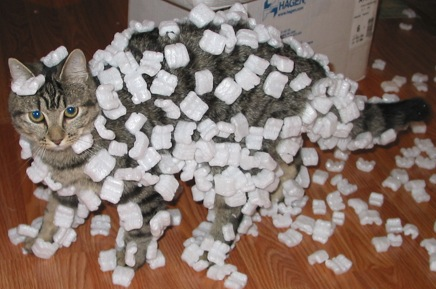
\includegraphics[height=0.36\textheight]{tribocat}
\end{figure}

\slidebibliography{
\slidebibentry{Wiki-N}{\url{https://en.wikipedia.org/wiki/Natural_number}}
\slidebibentry{Triboelectric-cat}{By Original image: Sean McGrath from Saint John, NB, CanadaDerived image: Black Rainbow 999 - This file has been extracted from another file, CC BY 2.0, \url{https://commons.wikimedia.org/w/index.php?curid=60287175}}
}
\end{frame}}

\begin{frame}{Missing features}
\begin{itemize}
\item You can refer to items in previous slides \slidecite{Triboelectric-cat}, \slidecite{Adams1979} but they don't currently appear to the bottom of the slide.
\item You can't currently get a list of all references e.g. to be displayed once more in the end of the presentation.
\item This thing is implemented as a glorified enumerate environment, with a custom counter. It's really dead simple so feel free to improve it further.
\end{itemize}

\end{frame}

\end{document}
